% -------------------------------------------------------------------
% Document setup
% -------------------------------------------------------------------
\documentclass[a4paper,12pt,oneside,spanish]{book}
\usepackage{babel}
\usepackage{styles}
\usepackage{tabularx}
\usepackage{titlesec}
\usepackage{float}

\titleformat{\section}[block]
  {\bfseries\Large}
  {\thesection.}
  {0.5em}
  {} % título sin adornos
  [\vspace{0.3ex}\titlerule]

\titleformat{\subsection}[block]
  {\bfseries\large}
  {\thesubsection.}
  {0.5em}
  {}

\begin{document}

    \frontmatter
    
    \begin{titlepage}
        \begin{center}
            
            \begin{center}
                
\includegraphics[width=2cm]{../resources/UNSL.png}\hspace{1cm}%
                
\includegraphics[width=2cm]{../resources/Dpto Informática.png}
            \end{center}
            \vspace{1cm}
            {\LARGE Universidad Nacional de San Luis\\[0.5cm]
            Departamento de Informática\\[1.2cm]
            }
            \linespread{1.2}\huge{

                %%%%%%%%%%%%%%%%%%%%%%%%%%%%
                % Project Title
                %%%%%%%%%%%%%%%%%%%%%%%%%%%%
                \textbf{\textit{Proyecto Final Integrador\\Sistemas Distribuidos y Paralelos}}
                \bigbreak%

                \textit{Procesamiento de Imágenes}
                
            }
            \linespread{1}~\\[1.2cm]
            
            {\Large
               
                %%%%%%%%%%%%%%%%%%%%%%%%%%%%
                % Authors
                %%%%%%%%%%%%%%%%%%%%%%%%%%%%
                
                \bigbreak%
                Facundo Nicolás Farias Lozano\\
                Franco Sarubbi
            }
            
            \linespread{1}~\\[1.2cm]

            {\large
                \emph{Profesores:}\\
                    Dra. María Fabiana Piccoli\\
                    Lic. Cesar Ochoa\\[0.5cm]
                    
                \emph{Ingeniería en Computación --- Ingeniería en Informática}\\

                
                \emph{2026}
            }
            

            \date{2025}
        \end{center}
    \end{titlepage}
    \pagestyle{plain}

    
    % -------------------------------------------------------------------
    % List of Abbreviations
    % -------------------------------------------------------------------
    \chapter*{Lista de Abreviaturas}
\addcontentsline{toc}{chapter}{Lista de Abreviaturas}

\begin{abbrv}
    \item[\textbf{HPC}] \textit{High Performance Computing} --- Computación de alto rendimiento.
    \item[\textbf{LUT}] \textit{Lookup Table} --- Tabla de búsqueda precalculada.
    \item[\textbf{NUMA}] \textit{Non-Uniform Memory Access} --- Arquitectura de acceso no uniforme a memoria.
    \item[\textbf{1D}] Unidimensional.
    \item[\textbf{2D}] Bidimensional.
\end{abbrv}


    % -------------------------------------------------------------------
    % Contents
    % -------------------------------------------------------------------
    \tableofcontents
    %%%%%%%%%%%%%%%%%%%%%%%%%%%%%%%%%%%%%%%%%%%%%%%%%%%%%%%%%%%%%%%%%%%%%%%%
    %%  Main chapters and sections                                        %%  
    %%%%%%%%%%%%%%%%%%%%%%%%%%%%%%%%%%%%%%%%%%%%%%%%%%%%%%%%%%%%%%%%%%%%%%%%
    \mainmatter%
    
    \chapter{Introducción}

El presente trabajo práctico integrador tiene como objetivo principal comprender y aplicar la problemática asociada al diseño e implementación de sistemas paralelos eficientes. Como caso de estudio empírico, se plantea el desarrollo de una aplicación de procesamiento de imágenes capaz de generar un efecto de \textit{Cartoon} a partir de una fotografía original. Para lograr este efecto visual sobre una matriz de píxeles, se debe construir un pipeline de transformaciones espaciales que incluye:
\begin{enumerate}
    \item Conversión de la imagen a escala de grises.
    \item Aplicación de filtros de convolución matemática para suavizado y detección de bordes.
    \item Reducción de la paleta de colores mediante posterización.
    \item Fusión de estos elementos.
\end{enumerate}


Con el fin de analizar cómo se adaptan estos algoritmos a diferentes arquitecturas de hardware, el proyecto propone resolver el problema mediante cuatro enfoques de programación distintos:

\begin{enumerate}
    \item \textbf{Modelo Secuencial:} Implementación base ejecutada en un único hilo de control, la cual sirve como punto de referencia algorítmico y métrico.
    
    \item \textbf{Modelo de Memoria Distribuida (MPI):} Versión paralela donde la carga de trabajo (el dominio de la imagen) se divide entre múltiples procesos independientes que no comparten memoria y deben coordinarse mediante el paso explícito de mensajes a través de la red.
    
    \item \textbf{Modelo de Memoria Compartida (OpenMP):} Implementación orientada a explotar arquitecturas multinúcleo dentro de un mismo nodo computacional, utilizando múltiples hilos de ejecución que comparten el mismo espacio de direccionamiento lógico.
    
    \item \textbf{Modelo Paralelo Híbrido:} Arquitectura avanzada que integra ambos paradigmas, utilizando MPI para la comunicación y distribución del trabajo a gran escala entre distintos nodos de un clúster, y OpenMP para maximizar el poder de cómputo local dentro de cada nodo.
\end{enumerate}

Finalmente, se evalúan métricas clave de la computación de alto rendimiento, tales como el \textit{Speedup} y la \textit{Eficiencia}. Las pruebas de benchmarking se realizan sometiendo al sistema a diferentes niveles de estrés computacional, variando la resolución de las imágenes (desde $800 \times 800$ hasta $5000 \times 5000$ píxeles), el tamaño de las matrices de convolución (filtros de $3 \times 3$ y $5 \times 5$) y los rangos de posterizado, con el objetivo de establecer conclusiones fundamentadas sobre la viabilidad y escalabilidad de cada paradigma.
    \chapter{Diseño e Implementación de los Algoritmos}

En este capítulo se detalla el proceso de ingeniería de software llevado a cabo para construir el pipeline de procesamiento de imágenes tipo \textit{Cartoon}. Como cimiento tecnológico para todas las implementaciones, se utilizó el lenguaje C por su cercanía al hardware y control explícito de la memoria, apoyado por la librería \texttt{stb\_image} para la decodificación y codificación eficiente de las imágenes.

La evolución del sistema se abordó de manera incremental. En primer lugar, se desarrolló una solución algorítmica puramente secuencial para validar la corrección de los filtros espaciales y establecer una línea base de tiempos. A partir de este núcleo validado, el código fue refactorizado y adaptado a tres paradigmas paralelos distintos: memoria compartida (OpenMP), memoria distribuida (MPI) y una aproximación híbrida (MPI + OpenMP). A continuación, se exponen las decisiones de diseño crítico, las estrategias de división de datos y los mecanismos de sincronización adoptados en cada una de estas iteraciones.


%--------------------------------------------------------------------
\section{El algoritmo secuencial}

La versión secuencial constituye el punto de partida del proyecto y cumple un doble propósito: por un lado, sirve como referencia funcional sobre la cual se validan los resultados de las versiones paralelas (asegurando que produzcan exactamente la misma imagen de salida); y por otro, es la base sobre la cual se calculan las métricas de speedup y eficiencia de las demás implementaciones.

\subsection{Gestión de Memoria en un Arreglo Unidimensional}

Una de las primeras decisiones de diseño fue la representación interna de la imagen. En lugar de modelarla como una matriz bidimensional (un arreglo de arreglos), se optó por aplanar la imagen en un único arreglo unidimensional y contiguo en memoria, de tamaño $\mathit{width} \times \mathit{height} \times \mathit{channels}$. Esta decisión no es meramente estética: al utilizar la función \texttt{stb\_image} para cargar la imagen, ésta ya entrega los datos en este formato, y mantenerlo así evita copias innecesarias y maximiza la localidad espacial. Cuando el procesador necesita leer un píxel, en realidad trae consigo a la memoria caché todo un bloque contiguo de píxeles vecinos, lo que reduce drásticamente la cantidad de accesos a la memoria RAM principal.

Para acceder a un píxel ubicado en la coordenada $(x, y)$ de la imagen, se calcula su posición dentro del arreglo unidimensional mediante la fórmula:

\begin{equation}
\label{eq:idx}
idx = y \times \mathit{width} + x
\end{equation}

A este índice base hay que multiplicarlo (o sumarle el desplazamiento correspondiente) según la cantidad de canales de color, dado que cada píxel ocupa varias posiciones consecutivas en el arreglo (3~posiciones para imágenes RGB). Este cálculo de índice es la operación más repetida de todo el programa, ya que se ejecuta dentro de cada bucle de procesamiento de la imagen, y por eso se mantuvo lo más simple y directo posible, evitando operaciones costosas dentro de los bucles internos.


\subsection{Flujo del Pipeline de Procesamiento}

El programa secuencial respeta un orden estricto de ejecución de los distintos filtros, ya que cada etapa depende del resultado de la anterior y alterar este orden produce resultados visualmente incorrectos. El pipeline implementado sigue la siguiente secuencia:

\begin{enumerate}
    \item \textbf{Conversión a Escala de Grises:} A partir de la imagen original a color, se genera una copia en escala de grises utilizando la fórmula de luminancia ponderada, ya que esta es la que mejor representa la percepción de brillo del ojo humano:
    \begin{equation}
    \label{eq:luminancia}
    L = 0.299 \cdot R + 0.587 \cdot G + 0.114 \cdot B
    \end{equation}
    
    \item \textbf{Borroneado (Box Blur):} Sobre la imagen en escala de grises se aplica un filtro espacial de convolución, de tamaño configurable $3 \times 3$ o $5 \times 5$, que suaviza la imagen eliminando ruido de alta frecuencia. Este paso es indispensable antes de detectar bordes, ya que sin él el detector confundiría el ruido propio de la fotografía con contornos reales.
    
    \item \textbf{Detección de Bordes (Sobel):} Sobre la imagen ya borroneada se aplica el filtro de Sobel, que aproxima el gradiente de intensidad utilizando dos kernels (uno horizontal y otro vertical) y obtiene la magnitud del borde mediante la suma de los valores absolutos ($|G_x| + |G_y|$), evitando así el cálculo costoso de raíces cuadradas. Los kernels de Sobel estándar utilizados son:
    \begin{equation}
    \label{eq:sobel_gx}
    G_x = \begin{bmatrix} -1 & 0 & 1 \\ -2 & 0 & 2 \\ -1 & 0 & 1 \end{bmatrix}
    \qquad
    G_y = \begin{bmatrix} -1 & -2 & -1 \\ 0 & 0 & 0 \\ 1 & 2 & 1 \end{bmatrix}
    \end{equation}
    Luego de obtener la magnitud, se aplica un umbral (\textit{threshold}) para decidir si el píxel corresponde a un borde (negro) o no (blanco/transparente).
    
    \item \textbf{Posterizado:} Sobre la imagen original a color (no sobre la versión gris ni borroneada) se aplica el posterizado mediante una tabla de búsqueda (LUT), reduciendo la cantidad de tonos por canal según el parámetro elegido por el usuario.
    
    \item \textbf{Fusión Final:} Por último, se combinan los resultados de las dos rutas anteriores. Se toma la imagen posterizada a color (que conserva los detalles cromáticos de la foto original) y se le ``estampan'' encima los píxeles negros detectados por el filtro de Sobel, generando así el efecto final de cartoon, con colores planos y contornos marcados.
\end{enumerate}

Este orden no es arbitrario: si se posteriza antes de calcular los bordes, o si se detectan bordes sobre la imagen original sin borronear, el resultado final perdería calidad o directamente sería incorrecto.


\subsection{Aislamiento de la Medición de Tiempos}

Para poder obtener métricas confiables de rendimiento, fue fundamental que la medición de tiempo se concentrara únicamente en el bloque de cálculo puro del pipeline, es decir, en la ejecución de los filtros descritos anteriormente. Para esto se utilizó la estructura \texttt{timeval} junto con la función \texttt{gettimeofday()}, tomando una marca de tiempo justo antes de comenzar la ejecución de los filtros y otra justo al finalizar, calculando luego la diferencia entre ambas.

Es importante destacar que todas las operaciones de Entrada/Salida (I/O), como la lectura de la imagen desde el disco mediante \texttt{stb\_image} y la escritura del resultado final, quedaron deliberadamente fuera de este bloque cronometrado. Esto se debe a que estas operaciones dependen fuertemente de factores externos al algoritmo en sí (velocidad del disco, sistema de archivos, buffers del SO) y su inclusión dentro de la medición introduciría ruido que distorsionaría las comparaciones de rendimiento entre la versión secuencial y las versiones paralelas. De esta manera, el tiempo medido refleja exclusivamente el costo computacional de los algoritmos de procesamiento de imágenes, que es lo que realmente nos interesa comparar.


%--------------------------------------------------------------------
%--------------------------------------------------------------------

\section{Paralelización en memoria compartida (OpenMP)}

Esta etapa consistió en paralelizar el código secuencial utilizando la especificación OpenMP, aprovechando que todos los núcleos de un mismo nodo comparten el mismo espacio de direcciones de memoria.


\subsection{Minimalismo}

Uno de los aspectos más destacables de esta etapa fue lo poco que tuvo que modificarse el código original para obtener paralelismo. Dado que el procesamiento de cada píxel es una operación independiente del resultado de los píxeles vecinos recién calculados, fue posible insertar directivas \texttt{\#pragma omp parallel for} directamente sobre los bucles más externos de cada función de filtrado, sin modificar la lógica de los filtros, permitiendo mantener una única base de código ``conceptual'' entre la versión secuencial y la paralela.

El siguiente fragmento de código ilustra la paralelización del filtro de borroneado, donde basta con añadir una directiva OpenMP sobre el bucle externo para distribuir las filas entre los hilos disponibles:

\begin{lstlisting}[language=C, caption={Paralelización del filtro Box Blur con OpenMP}, label=list:blur_omp]
void apply_blur(unsigned char *img_in, unsigned char *img_out,
                int width, int height, int filter_size) {
    int offset = filter_size / 2;
    int num_elements = filter_size * filter_size;

    #pragma omp parallel for schedule(static) // Directiva OpenMP
    for (int i = 0; i < width * height; i++) {
        img_out[i] = 0;
    }

    #pragma omp parallel for schedule(static) // Directiva OpenMP
    for (int y = offset; y < height - offset; y++) {
        for (int x = offset; x < width - offset; x++) {
            int sum = 0;
            for (int ky = -offset; ky <= offset; ky++) {
                for (int kx = -offset; kx <= offset; kx++) {
                    int idx = (y + ky) * width + (x + kx);
                    sum += img_in[idx];
                }
            }
            int final_idx = y * width + x;
            img_out[final_idx] = (unsigned char)(sum / num_elements);
        }
    }
}
\end{lstlisting}


\subsection{Planificación Estática}

Al momento de elegir la política de planificación del bucle paralelo, se optó por \texttt{schedule(static)} en lugar de las alternativas dinámicas (\texttt{dynamic} o \texttt{guided}). Esta decisión se basa en la naturaleza misma del problema: el procesamiento de una imagen es un caso de carga de trabajo completamente predecible y uniforme, ya que el costo computacional de aplicar un filtro a un píxel es idéntico para cualquier píxel de la imagen.

De esta manera, la planificación estática divide el espacio total de iteraciones en bloques grandes y contiguos, asignándolos de manera fija a cada hilo desde el inicio, por lo que se elimina por completo el \textit{overhead} de tener que consultar al planificador en tiempo de ejecución para repartir nuevas tandas de trabajo, como ocurriría con una planificación dinámica. Además, al estar los bloques de cada hilo separados por una gran cantidad de memoria, se evita por diseño el problema de \textit{false sharing} (donde distintos hilos escriben en variables que comparten la misma línea de caché), por lo que no fue necesario recurrir a mecanismos de sincronización costosos como \texttt{\#pragma omp critical} dentro de los bucles de procesamiento.


\subsection{Prevención de Condiciones de Carrera}

La lectura de la imagen fuente y la escritura sobre la imagen de destino se realizan sobre arreglos compartidos por todos los hilos, pero existen ciertas variables auxiliares que sí representan un riesgo de condición de carrera si se manejan incorrectamente. Consideremos el cálculo del filtro de Sobel, donde para cada píxel se necesitan acumular los resultados parciales de la convolución horizontal y vertical en variables como \texttt{sumX} y \texttt{sumY}.

La solución adoptada fue declarar estas variables acumuladoras dentro del cuerpo del bucle paralelo, es decir, en su ámbito local. De esta forma, cada hilo obtiene su propia copia privada de \texttt{sumX} y \texttt{sumY} en cada iteración, evitando que distintos hilos lean o escriban sobre la misma variable acumuladora al mismo tiempo. Esta privatización por hilo es automática gracias al alcance (\textit{scope}) de las variables en C, y no requirió el uso explícito de cláusulas como \texttt{private()} ni de directivas de sincronización adicionales, manteniendo el código simple y correcto.


\subsection{Optimización de Memoria mediante First-Touch (NUMA)}

En la implementación original, antes de ejecutar la lógica de cada filtro, se recorre el arreglo de salida (\texttt{img\_out}) inicializando todas sus posiciones en cero (\texttt{img\_out[i] = 0}). Esta inicialización, al igual que el cálculo principal, también fue envuelta dentro de una región paralela con \texttt{\#pragma omp parallel for}.

La razón detrás de esto tiene que ver con la política de gestión de memoria del SO en arquitecturas con múltiples sockets de CPU Non Uniform Memory Access (NUMA). En estos sistemas, las páginas de memoria física no quedan asignadas a un nodo NUMA en particular en el momento del \texttt{malloc}, sino recién en el momento del primer acceso efectivo a esa memoria (política conocida como \textit{first-touch}). Si la inicialización en cero se hiciera de forma secuencial (solo por el hilo principal), todas las páginas de memoria del arreglo quedarían asignadas físicamente al nodo NUMA donde corre dicho hilo. Luego, cuando los demás hilos de trabajo (ubicados en otros núcleos o sockets) intenten escribir sus resultados durante el cálculo pesado del filtro, tendrían que acceder a memoria física ubicada en un nodo NUMA remoto, lo que introduce una penalización de latencia.

Al paralelizar también el bucle de inicialización, cada hilo realiza el \textit{first-touch} sobre el bloque de memoria que luego le corresponderá procesar, forzando al SO a repartir las páginas físicas de memoria entre los distintos nodos NUMA de manera alineada con la distribución del cómputo. Si bien esta optimización no afecta la corrección del resultado (el programa funciona igual sin ella), sí resulta relevante para que las curvas de speedup y eficiencia escalen correctamente al ejecutarse en los nodos multi-socket del clúster.


\subsection{LUT Secuencial}

Por último, cabe justificar por qué la función \texttt{generate\_lut}, encargada de precalcular la tabla de búsqueda utilizada para el posterizado, se mantuvo sin paralelizar. Esta función recorre únicamente las 256~posiciones posibles de un canal de color (rango de 0 a 255), calculando una sola vez el valor posterizado correspondiente a cada nivel de intensidad.

\begin{lstlisting}[language=C, caption={Generación de la LUT para posterizado}, label=list:generate_lut]
void generate_lut(unsigned char lut[256], int levels) {
    if (levels < 2) levels = 2;
    int step = 256 / levels;
    for (int i = 0; i < 256; i++) {
        int bucket = i / step;
        if (bucket >= levels) bucket = levels - 1;
        lut[i] = (unsigned char)(bucket * (255.0 / (levels - 1)));
    }
}
\end{lstlisting}

Dado que crear un equipo de hilos en OpenMP no es una operación gratuita (implica cierto \textit{overhead} de sincronización al iniciar y finalizar la región paralela), paralelizar un bucle de apenas 256~iteraciones es más costoso que el cálculo en sí. Por este motivo, se decidió dejar esta función ejecutándose de forma puramente secuencial, reservando el paralelismo para las operaciones de filtros aplicados sobre los millones de píxeles de la imagen.


%--------------------------------------------------------------------
\section{Paralelización en memoria distribuida (MPI)}

En esta etapa el foco estuvo en extender el procesamiento más allá de los límites de un solo nodo, distribuyendo la carga de trabajo entre múltiples procesos independientes mediante el estándar MPI.


\subsection{Descomposición en bloques 1D}

La primera decisión de diseño fue cómo dividir la imagen entre los distintos procesos. Se descartó una descomposición en bloques 2D, ya que, si bien teóricamente minimiza la relación entre el perímetro y el área de cada subdominio, en la práctica requeriría transmitir columnas de píxeles no contiguas en memoria. Esto obligaría a empaquetar y desempaquetar constantemente datos dispersos, generando así \textit{overhead} y anulando cualquier beneficio.

Por este motivo, se optó porque cada proceso reciba un bloque contiguo de filas completas de la imagen (descomposición de dominio unidimensional o 1D). De esta manera, el proceso raíz puede repartir estos bloques directamente mediante punteros de memoria sin necesidad de ningún empaquetado adicional, maximizando así el rendimiento.

Sin embargo, tenemos un problema práctico: la altura de la imagen rara vez es perfectamente divisible por la cantidad de procesos disponibles. Para resolver esto, el proceso raíz calcula cuántas filas le corresponden a cada proceso mediante una división entera, y su resto, el cual se distribuye repartiendo una fila extra a los primeros procesos hasta agotarlo. Con esto se logra que la diferencia de carga entre el proceso que más filas recibe y el que menos recibe sea, como máximo, de una sola fila:

\begin{lstlisting}[language=C, caption={Descomposición de dominio 1D con distribución balanceada}, label=list:domain_decomp]
int base_rows = height / size;
int remainder = height % size;
for (int i = 0; i < size; i++) {
    row_counts[i] = base_rows + (i < remainder ? 1 : 0);
}
\end{lstlisting}

Para implementar esta distribución balanceada, fue necesario el uso de las funciones \texttt{MPI\_Scatterv} y \texttt{MPI\_Gatherv}, en lugar de \texttt{MPI\_Scatter} y \texttt{MPI\_Gather}, que únicamente permiten repartir fragmentos de igual tamaño.


\subsection{Mecanismo de Halo Exchange (Zonas Fantasma)}

El mayor desafío de esta etapa fue al momento de aplicar los filtros de borroneado y Sobel. El problema es el siguiente: para calcular el nuevo valor de un píxel ubicado en la primera o última fila del bloque asignado a un proceso, el filtro necesita leer los valores de las filas vecinas, que físicamente se encuentran en la memoria de otro proceso, por lo que esta información no está disponible directamente.

Para resolver este aislamiento, cada proceso reserva, además de las filas que efectivamente le corresponden procesar, una cantidad adicional de filas ``fantasma'' (\textit{halo}) en los extremos superior e inferior de su bloque local. El tamaño de este halo no es fijo, sino que se calcula dinámicamente en función del tamaño del kernel de convolución utilizado, mediante la expresión:

\begin{equation}
\label{eq:halo_size}
\mathit{halo\_size} = \left\lfloor \frac{\mathit{filter\_size}}{2} \right\rfloor
\end{equation}

Es decir, un filtro de $3 \times 3$ requiere un halo de 1~fila de espesor, mientras que un filtro de $5 \times 5$ requiere un halo de 2~filas.

Antes de comenzar el procesamiento propiamente dicho, todos los procesos participan de una fase de comunicación destinada a llenar estas zonas fantasma con las filas reales correspondientes de sus vecinos. Cabe destacar que los procesos en los extremos del dominio (el primero y el último) se comportan de manera distinta a los procesos intermedios, ya que los procesos extremos solo tienen un vecino de un lado, y del otro lado simplemente no existe información que recibir.


\subsection{Comunicación Segura y Prevención de Deadlocks}

Para implementar este intercambio de filas fantasma se diseñó la función modular \texttt{halo\_exchange}, que encapsula toda la lógica de comunicación entre vecinos. Un enfoque es utilizar el par de llamadas \texttt{MPI\_Send} y \texttt{MPI\_Recv} de manera secuencial; sin embargo, si todos los procesos intentan enviar datos al mismo tiempo sin que ninguno haya publicado aún un buffer de recepción, obtenemos un \textit{deadlock}. Para evitar este riesgo, la función \texttt{halo\_exchange} se implementó utilizando la primitiva \texttt{MPI\_Sendrecv}, que combina en una sola llamada una operación de envío y una de recepción de forma simultánea, dejando que la propia biblioteca de MPI se encargue internamente de coordinar el intercambio.

El intercambio completo se realiza en dos pasos simétricos: primero un intercambio ``ascendente'', donde cada proceso envía sus filas reales superiores a su vecino de arriba y recibe de él sus filas fantasma superiores; y luego un intercambio ``descendente'', análogo pero en sentido contrario, con el vecino de abajo.

\begin{lstlisting}[language=C, caption={Función de intercambio de halos con \texttt{MPI\_Sendrecv}}, label=list:halo_exchange]
void halo_exchange(unsigned char *extended_buf, int local_rows,
                   int width, int halo_size, int ghost_top,
                   int ghost_bottom, int rank, int size) {

    int up = (rank > 0) ? rank - 1 : MPI_PROC_NULL;
    int down = (rank < size - 1) ? rank + 1 : MPI_PROC_NULL;
    int halo_bytes = halo_size * width;

    // Paso 1: intercambio descendente
    MPI_Sendrecv(
        extended_buf + (ghost_top + local_rows - halo_size)*width,
        halo_bytes, MPI_UNSIGNED_CHAR, down, 0,
        extended_buf + (ghost_top + local_rows)*width,
        ghost_bottom * width, MPI_UNSIGNED_CHAR, down, 1,
        MPI_COMM_WORLD, MPI_STATUS_IGNORE);

    // Paso 2: intercambio ascendente
    MPI_Sendrecv(
        extended_buf + ghost_top * width,
        halo_bytes, MPI_UNSIGNED_CHAR, up, 1,
        extended_buf,
        ghost_top * width, MPI_UNSIGNED_CHAR, up, 0,
        MPI_COMM_WORLD, MPI_STATUS_IGNORE);
}
\end{lstlisting}

Finalmente, para evitar tener que escribir lógica condicional especial (\texttt{if/else}) que distinga el comportamiento de los procesos extremos (\textit{rank}~0 y el último \textit{rank}), se aprovechó el destino virtual \texttt{MPI\_PROC\_NULL} que ofrece MPI. Cuando un proceso extremo no tiene un vecino real hacia un lado, simplemente se configura ese ``vecino'' como \texttt{MPI\_PROC\_NULL}, permitiendo que la operación se complete sin realizar ninguna transferencia real de datos.


%--------------------------------------------------------------------
\section{Arquitectura híbrida (MPI + OpenMP)}

La última versión del proyecto combina los dos modelos de paralelismo desarrollados anteriormente, buscando aprovechar la jerarquía física de un clúster moderno: por un lado, múltiples nodos conectados por una red, y por otro lado, dentro de cada nodo, múltiples núcleos de CPU que comparten memoria.


\subsection{Nivel de Soporte Multi-Hilo}

Al combinar MPI con multithreading dentro de un mismo proceso, surge un riesgo adicional: si varios hilos de OpenMP intentaran invocar funciones de MPI de manera simultánea, el estado interno de la biblioteca de MPI podría corromperse. Para evitar esto, MPI ofrece distintos niveles de soporte de hilos, que se solicitan explícitamente mediante la función \texttt{MPI\_Init\_thread} (en lugar del clásico \texttt{MPI\_Init}).

Para este proyecto se eligió el nivel \texttt{MPI\_THREAD\_FUNNELED}. Bajo esta política, la aplicación puede tener múltiples hilos en ejecución, pero únicamente el \textit{Master Thread} tiene permitido realizar llamadas a funciones de MPI. El resto de los hilos de trabajo (\textit{Workers}) quedan restringidos a operar exclusivamente sobre la RAM local del nodo, sin ningún tipo de acceso a la red.


\subsection{Flujo de Trabajo Jerárquico}

La aplicación híbrida orquesta ambos modelos de paralelismo de manera secuencial dentro de cada ``ronda'' de procesamiento, alternando entre comunicación de red y cómputo local. Primero, a nivel de MPI, el proceso raíz divide la imagen completa en bloques de filas (utilizando lógica de \texttt{MPI\_Scatterv} descripta anteriormente) y los distribuye entre los distintos procesos, uno por nodo. Inmediatamente después, todos los procesos participan del intercambio de halos (\textit{halo exchange}) descrito anteriormente, para que cada uno tenga en su memoria local todas las filas (propias y fantasma) que va a necesitar.

Una vez que esta fase de sincronización de red finaliza y la memoria local de cada proceso queda completamente coherente, el \textit{Master Thread} de cada proceso invoca a su equipo de hilos OpenMP mediante las directivas \texttt{\#pragma omp parallel for}. A partir de este punto, todos los threads del nodo trabajan en simultáneo sobre la porción de imagen que le fue asignada a ese proceso MPI, aplicando los filtros de borroneado, Sobel y posterizado sobre sus filas correspondientes. Al finalizar el procesamiento, el proceso raíz recolecta los resultados de todos los nodos mediante \texttt{MPI\_Gatherv} para ensamblar la imagen final.

De esta manera, la red solo se utiliza para repartir la imagen, intercambiar halos y recolectar resultados, mientras que la gran mayoría del tiempo de cómputo se realiza de forma local, aprovechando al máximo el ancho de banda de memoria compartida dentro de cada nodo.
    \chapter{Análisis de Desempeño y Benchmarking}

Para evaluar de forma rigurosa el rendimiento de las cuatro implementaciones desarrolladas, se diseñó un benchmarking script que somete a cada versión del programa a seis configuraciones distintas de trabajo computacional, combinando tres resoluciones de imagen ($800 \times 800$, $2000 \times 2000$ y $5000 \times 5000$~píxeles) con dos perfiles de filtrado: un \textit{perfil liviano} (filtro de $3 \times 3$ con 3~niveles de posterizado) y un \textit{perfil pesado} (filtro de $5 \times 5$ con 9~niveles de posterizado). Cada configuración se ejecutó durante 10~iteraciones consecutivas para obtener muestras estadísticamente representativas. Las pruebas se realizaron sobre un clúster donde OpenMP utilizó 32~núcleos dentro de un único nodo, mientras que MPI y la versión Híbrida emplearon 128~núcleos distribuidos en 4~nodos ($4\ \mathit{nodos} \times 32\ \mathit{cores}$).

A continuación se presenta el análisis detallado de cada escenario, seguido de una comparación general, las curvas de \textit{Speedup} y \textit{Eficiencia}, y un estudio de escalabilidad en función de la cantidad de hilos.


%--------------------------------------------------------------------
\section{Imagen de \texorpdfstring{$800 \times 800$}{800x800} píxeles}

\subsection{Configuración: filtro \texorpdfstring{$3 \times 3$}{3x3}, 3 niveles}

\begin{figure}[H]
    \centering
    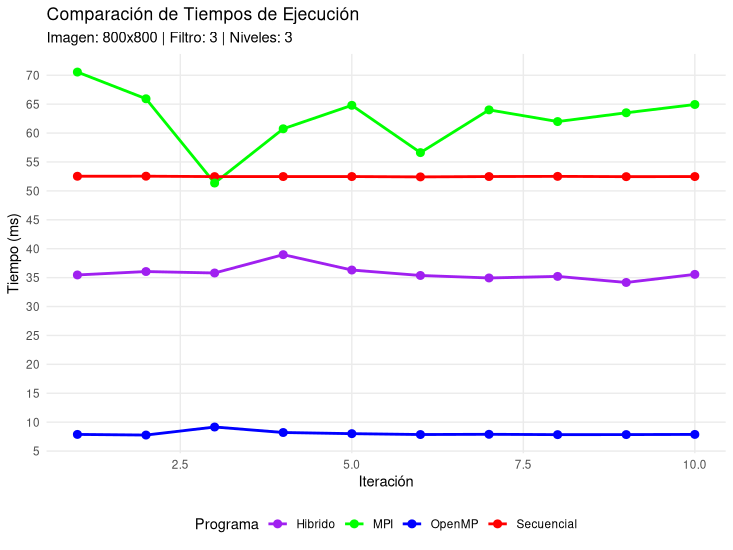
\includegraphics[width=0.85\textwidth]{../resources/800_3_3.png}
    \caption{Comparación de tiempos de ejecución --- Imagen $800 \times 800$, filtro $3 \times 3$, 3~niveles de posterizado.}
    \label{fig:800_3_3}
\end{figure}

En la configuración más liviana del benchmark, la carga computacional resulta extremadamente reducida: la versión secuencial completa el pipeline en aproximadamente 52~ms de forma estable a lo largo de las 10~iteraciones. OpenMP demuestra una aceleración notable, reduciendo los tiempos a cerca de 8~ms con una variabilidad mínima entre iteraciones. Sin embargo, la versión MPI exhibe el comportamiento más desfavorable de los cuatro modelos, con tiempos que oscilan entre 51~ms y 71~ms, superando incluso a la versión secuencial en la mayoría de las iteraciones. Este resultado evidencia que, para un volumen de datos reducido ($800 \times 800 = 640{.}000$~píxeles), el \textit{overhead} inherente a la comunicación por red (distribución mediante \texttt{MPI\_Scatterv}, intercambio de halos y recolección con \texttt{MPI\_Gatherv}) supera al beneficio obtenido por la paralelización del cómputo entre los 128~núcleos. La versión Híbrida se posiciona en un punto intermedio, con tiempos alrededor de 35~ms: si bien logra reducir el tiempo respecto de la versión secuencial gracias al cómputo paralelo interno con OpenMP, aún arrastra la penalización de la coordinación entre los 4~nodos MPI.


\subsection{Configuración: filtro \texorpdfstring{$5 \times 5$}{5x5}, 9 niveles}

\begin{figure}[H]
    \centering
    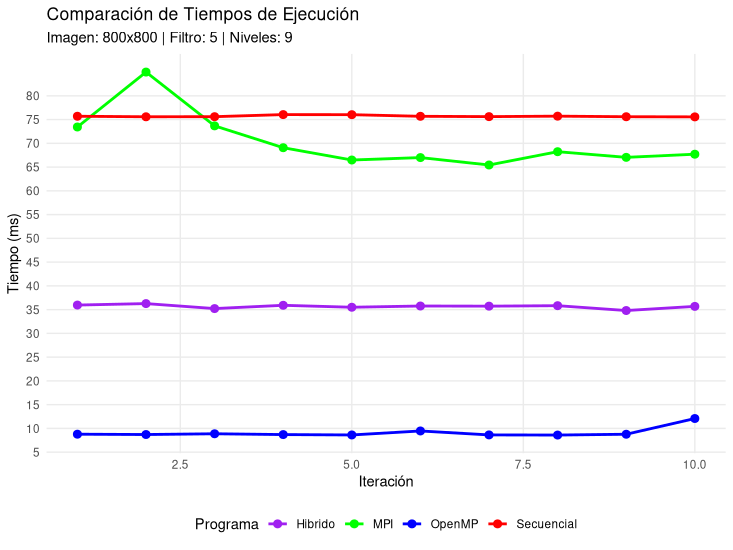
\includegraphics[width=0.85\textwidth]{../resources/800_5_9.png}
    \caption{Comparación de tiempos de ejecución --- Imagen $800 \times 800$, filtro $5 \times 5$, 9~niveles de posterizado.}
    \label{fig:800_5_9}
\end{figure}

Al incrementar la complejidad del filtrado (kernel de $5 \times 5$, que implica 25~operaciones por píxel en lugar de 9, y 9~niveles de posterizado), los tiempos secuenciales ascienden a aproximadamente 76~ms. OpenMP continúa liderando con tiempos cercanos a 9~ms, prácticamente sin degradación respecto de la configuración anterior. La versión MPI se mantiene cercana a los tiempos del modelo secuencial, oscilando entre 65~ms y 85~ms, pero por debajo respecto de la línea base secuencial en la mayoría de iteraciones, logrando una aceleración positiva y justificando el costo de la comunicación entre los 128~procesos. La versión Híbrida mantiene su comportamiento estable alrededor de 36~ms, confirmando que el cuello de botella en esta resolución no es el cómputo sino la latencia de comunicación entre nodos.



%--------------------------------------------------------------------
\section{Imagen de \texorpdfstring{$2000 \times 2000$}{2000x2000} píxeles}

\subsection{Configuración: filtro \texorpdfstring{$3 \times 3$}{3x3}, 3 niveles}

\begin{figure}[H]
    \centering
    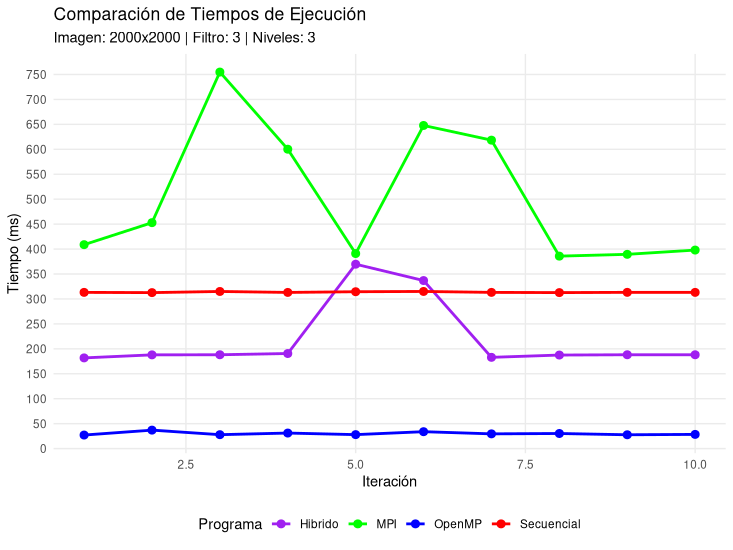
\includegraphics[width=0.85\textwidth]{../resources/2000_3_3.png}
    \caption{Comparación de tiempos de ejecución --- Imagen $2000 \times 2000$, filtro $3 \times 3$, 3~niveles de posterizado.}
    \label{fig:2000_3_3}
\end{figure}

Con una imagen de resolución intermedia ($2000 \times 2000 = 4{.}000{.}000$~píxeles), las diferencias entre los paradigmas comienzan a acentuarse. La versión secuencial se mantiene estable aproximadamente en torno a 315~ms. OpenMP reduce drásticamente este tiempo a un rango de 25--40~ms, demostrando una escalabilidad sólida al aumentar el tamaño del problema. La versión MPI, en cambio, tiene una alta inestabilidadm, con tiempos que fluctúan entre 385~ms y 755~ms, y con picos que casi duplican el tiempo secuencial; esta variabilidad se le puede atribuir a la congestión de red. La versión Híbrida presenta un comportamiento interesante: en la mayoría de las iteraciones se mantiene alrededor de 188~ms y por debajo de la línea base secuencial, pero en las iteraciones 5 y 6 se observan picos de hasta 370~ms, posiblemente causados por interferencia puntual en la red del clúster.


\subsection{Configuración: filtro \texorpdfstring{$5 \times 5$}{5x5}, 9 niveles}

\begin{figure}[H]
    \centering
    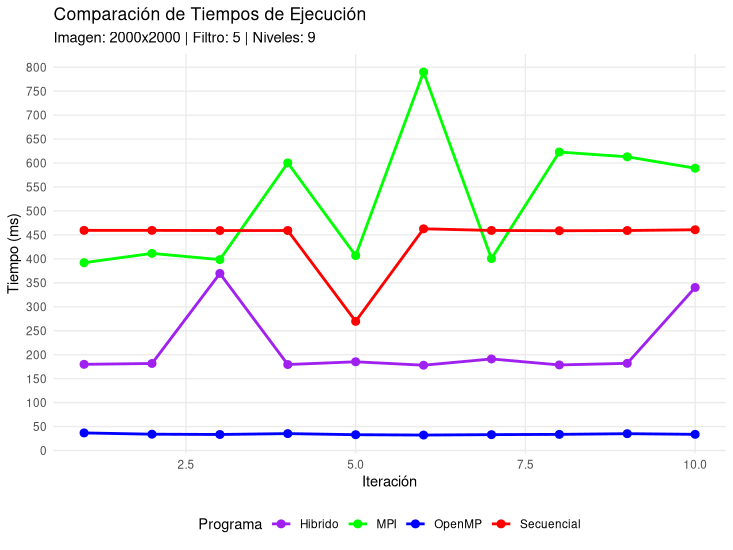
\includegraphics[width=0.85\textwidth]{../resources/2000_5_9.png}
    \caption{Comparación de tiempos de ejecución --- Imagen $2000 \times 2000$, filtro $5 \times 5$, 9~niveles de posterizado.}
    \label{fig:2000_5_9}
\end{figure}

El perfil pesado sobre la imagen de $2000 \times 2000$ eleva el tiempo secuencial a aproximadamente 460~ms, con un valor anómalo en la iteración~5 de 270~ms, probablemente causado por un efecto de caché favorable en esa ejecución particular. OpenMP mantiene tiempos consistentemente bajos entre 35~ms y 40~ms, demostrando que la mayor carga aritmética del kernel de $5 \times 5$ se paraleliza sin degradación apreciable. MPI presenta su peor comportamiento en esta configuración, con picos que alcanzan los 790~ms, practicamente duplicando el tiempo secuencial, y una dispersión considerable entre iteraciones (rango de 390~ms a 790~ms). La versión Híbrida se mantiene generalmente estable cerca de 180~ms, aunque nuevamente se observan picos esporádicos (iteraciones 3 y 10 por encima de 340~ms), coherentes con el patrón de interferencia de red observado.


%--------------------------------------------------------------------
\section{Imagen de \texorpdfstring{$5000 \times 5000$}{5000x5000} píxeles}

\subsection{Configuración: filtro \texorpdfstring{$3 \times 3$}{3x3}, 3 niveles}

\begin{figure}[H]
    \centering
    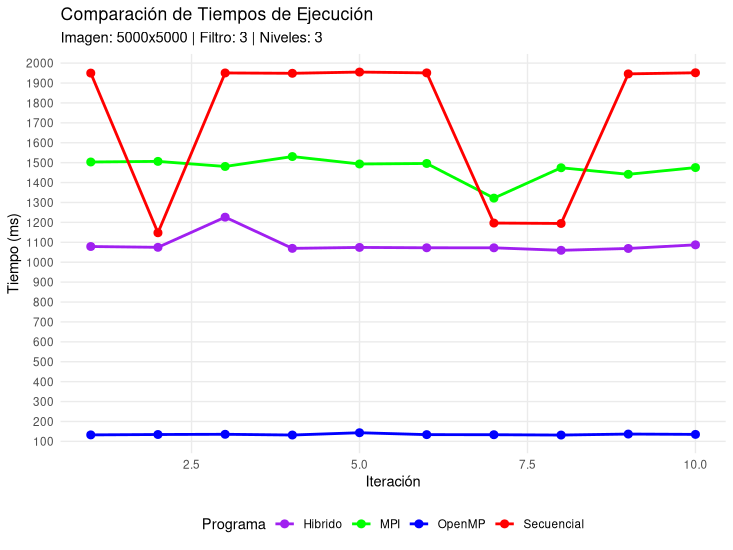
\includegraphics[width=0.85\textwidth]{../resources/5000_3_3.png}
    \caption{Comparación de tiempos de ejecución --- Imagen $5000 \times 5000$, filtro $3 \times 3$, 3~niveles de posterizado.}
    \label{fig:5000_3_3}
\end{figure}

Al alcanzar la resolución máxima del benchmark ($5000 \times 5000 = 25{.}000{.}000$~píxeles), el escenario cambia significativamente respecto de las resoluciones menores. La versión secuencial presenta tiempos alrededor de 1950~ms, con caídas a 1150--1200~ms en las iteraciones 2, 7 y 8 (atribuibles a efectos de caché). OpenMP continúa obteniendo los mejores tiempos, entre 130~ms y 140~ms. La observación más relevante en esta resolución es que MPI logra nuevamente superar a la versión secuencial con tiempos entre 1320~ms y 1530~ms, lo que indica que el volumen de cómputo de 25~millones de píxeles justifica el costo de la comunicación MPI. La versión Híbrida consolida su posición intermedia con tiempos alrededor de 1070~ms, superando tanto a la versión secuencial como a MPI, y confirmando que la reducción del tráfico de red (de 128 a solo 4~procesos MPI) combinada con el paralelismo local de OpenMP resulta una estrategia más eficiente que MPI puro.


\subsection{Configuración: filtro \texorpdfstring{$5 \times 5$}{5x5}, 9 niveles}

\begin{figure}[H]
    \centering
    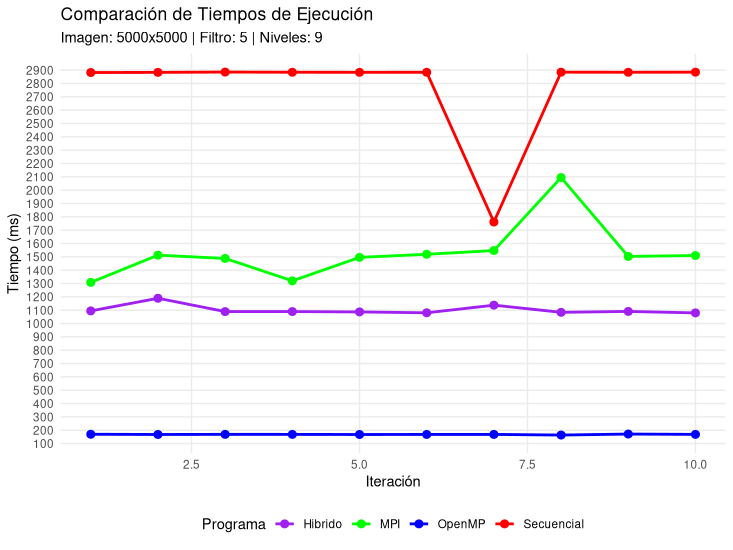
\includegraphics[width=0.85\textwidth]{../resources/5000_5_9.png}
    \caption{Comparación de tiempos de ejecución --- Imagen $5000 \times 5000$, filtro $5 \times 5$, 9~niveles de posterizado.}
    \label{fig:5000_5_9}
\end{figure}

La configuración más exigente del benchmark ($5000 \times 5000$ con kernel de $5 \times 5$ y 9~niveles) expone con máxima claridad la jerarquía de rendimiento entre las cuatro implementaciones. La versión secuencial alcanza los 2890~ms de forma estable, con una excepción en la iteración~7, que desciende a 1760~ms; nuevamente un caso atípico. OpenMP logra tiempos entre 160~ms y 170~ms; $10$ veces superior respecto del modelo secuencial. MPI mantiene tiempos entre 1310~ms y 1540~ms en la mayoría de las iteraciones, con un pico aislado de 2100~ms en la iteración~8, demostrando que, si bien la paralelización es efectiva a esta escala, la variabilidad introducida por la red sigue siendo un factor influyente. La versión Híbrida se estabiliza entre 1090~ms y 1190~ms, superando consistentemente tanto a la versión secuencial como a MPI puro, y posicionándose como la segunda opción más rápida después de OpenMP en un único nodo.


%--------------------------------------------------------------------
\section{Comparación General de Tiempos}

\begin{figure}[H]
    \centering
    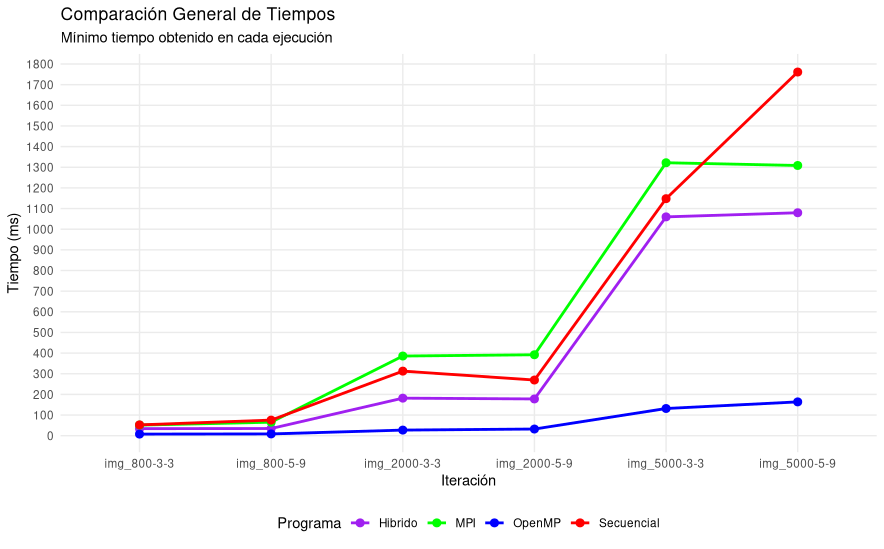
\includegraphics[width=0.9\textwidth]{../resources/Comp_General.png}
    \caption{Comparación general de tiempos --- Mínimo tiempo obtenido por cada implementación en las seis configuraciones de benchmark.}
    \label{fig:comp_general}
\end{figure}

La vista de los mejores tiempos obtenidos en cada configuración permite visualizar con claridad las tendencias de escalabilidad de cada paradigma. Para las resoluciones pequeñas ($800 \times 800$), los cuatro modelos operan en un rango temporal estrecho (entre 8~ms y 71~ms), donde la diferencia absoluta entre el mejor y el peor caso resulta poco significativa en términos prácticos. Sin embargo, a medida que la resolución crece, las curvas divergen drásticamente.

La versión Secuencial (línea roja) sirve como referencia superior, con un crecimiento lineal respecto del volumen de datos.

OpenMP (línea azul) se mantiene en la franja inferior del gráfico en todas las configuraciones, creciendo de forma suave y controlada: pasa de aproximadamente 8~ms en $800 \times 800$ a 160~ms en $5000 \times 5000$. Este crecimiento es proporcionalmente menor al aumento del volumen de datos, lo que demuestra una paralelización altamente eficiente dentro de un único nodo.

La versión Híbrida (línea morada) muestra un comportamiento intermedio consistente: su curva crece más lentamente que la de MPI, confirmando que reducir la cantidad de procesos MPI a solo 4 (uno por nodo) y delegar el paralelismo fino a OpenMP es una estrategia más escalable que utilizar MPI de forma exclusiva.

MPI (línea verde) exhibe la peor escalabilidad: si bien en algunas resoluciones sus tiempos superan a los de la versión secuencial, su curva crece de forma empinada y con alta variabilidad.


%--------------------------------------------------------------------
\section{Análisis de Speedup}

\begin{figure}[H]
    \centering
    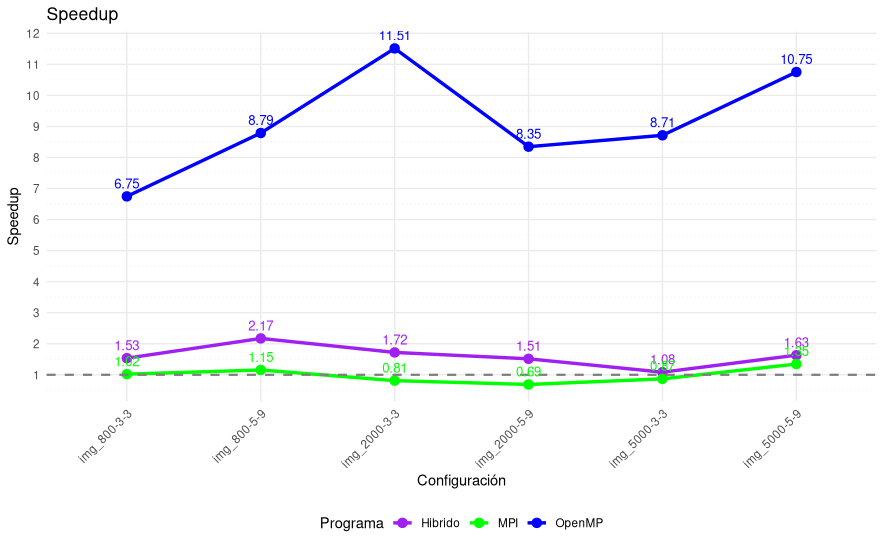
\includegraphics[width=0.9\textwidth]{../resources/Speedup.png}
    \caption{Speedup de las implementaciones paralelas respecto de la versión secuencial en las seis configuraciones de benchmark. La línea punteada indica $S = 1$ (sin aceleración).}
    \label{fig:speedup}
\end{figure}

Aquí podemos observar que OpenMP alcanza speedups considerablemente elevados durante todas las configuraciones, con un máximo de $11.51$ y un valor de $10.75$ en la configuración más exigente.

De MPI obtenemos el siguiente resultado: En tres configuraciónes obtiene ganancia (speedup mayor a 1), y en tres configuraciones no obtiene ganancia (speedup inferioir a 1), haciendo dificíl la elección de su implementación en un proyecto de esta escala.

La versión Híbrida logra speedups modestos comparados con OpenMP, pero superiores a MPI en todos los casos, oscilando entre $1.51$ y $2.17$. A pesar de ser resultados humildes, superan consistentemente la línea de $S = 1$, lo que demuestra que la combinación de ambos paradigmas resulta viable incluso cuando la escala del problema no favorece del todo a MPI puro.


%--------------------------------------------------------------------
\section{Análisis de Eficiencia}

\begin{figure}[H]
    \centering
    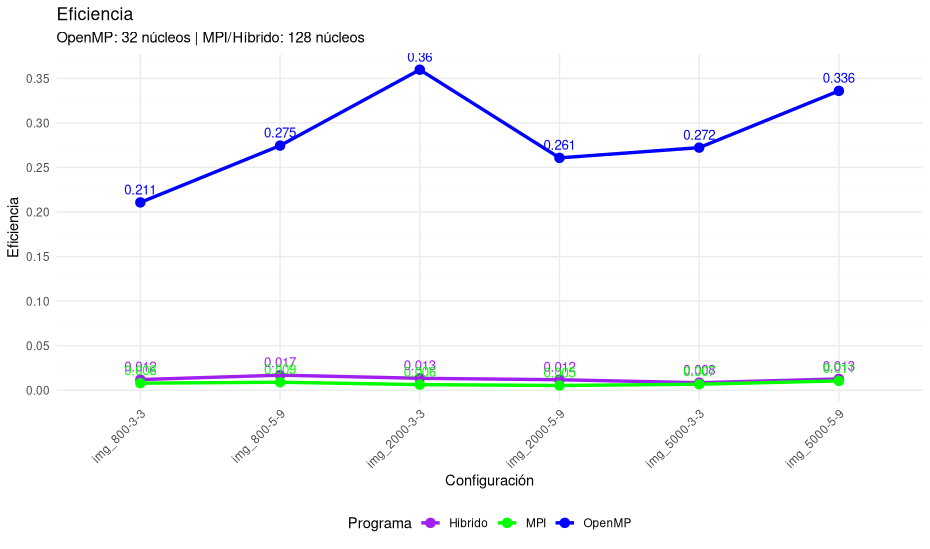
\includegraphics[width=0.9\textwidth]{../resources/Eficiencia.png}
    \caption{Eficiencia de las implementaciones paralelas. OpenMP utiliza 32~núcleos; MPI e Híbrido utilizan 128~núcleos.}
    \label{fig:eficiencia}
\end{figure}

Los resultados revelan una diferencia abismal en el aprovechamiento de los recursos. OpenMP, con 32~núcleos, alcanza eficiencias entre $0.211$ y $0.360$, lo que significa que entre el 21\% y el 36\% de la capacidad de cómputo se traduce en aceleración real.

En marcado contraste, MPI e Híbrido presentan eficiencias extremadamente bajas: entre $0{.}005$ y $0{.}017$ para MPI ($0{.}5\%$--$1{.}7\%$ de aprovechamiento) y entre $0{.}008$ y $0{.}017$ para Híbrido ($0{.}8\%$--$1{.}7\%$ de aprovechamiento). Estas cifras indican que la gran mayoría de los 128~núcleos asignados pasan una fracción dominante de su tiempo esperando comunicaciones de red, sincronizaciones de barrera o intercambios de halos, en lugar de realizar cómputo útil.

De este resultado podemos decir que: \textbf{Agregar más procesadores no siempre se traduce en mayor rendimiento} y, para este problema en particular, la configuración de 32~núcleos con memoria compartida (OpenMP) se posiciona como la opción más eficiente.


%--------------------------------------------------------------------
\section{Escalabilidad según Cantidad de Hilos}

Los análisis previos evaluaron el rendimiento de cada paradigma con una cantidad fija de unidades de procesamiento (32~hilos para OpenMP, 128~núcleos para MPI e Híbrido). Ahora nos toca observar cómo escala cada implementación al incrementar gradualmente los threads disponibles. Para ello, se diseñó un script el cuál varia la cantidad de hilos OpenMP utilizando la secuencia $\{1, 2, 4, 8, 16, 32\}$ (potencias de a dos), manteniendo fija la configuración computacionalmente más exigente del benchmark: imagen de $5000 \times 5000$~píxeles con filtro de $5 \times 5$ y 9~niveles de posterizado. ¿Por qué esta configuración? Maximizar el volumen de cómputo por píxel permite observar con mayor claridad la tendencia de escalabilidad.

Para la versión OpenMP, las 10~iteraciones de cada configuración se ejecutaron sobre un único nodo del clúster, variando exclusivamente el parámetro \texttt{-t} que controla la cantidad de threads. Para la versión Híbrida, se mantuvieron fijos los 4~procesos MPI (uno por nodo físico) y se varió la cantidad de hilos OpenMP internos de cada proceso. En ambos casos, el speedup se calculó de forma relativa a la ejecución con un único hilo del mismo programa ($S(p) = T(1) / T(p)$), lo que permite medir la ganancia neta atribuible exclusivamente al aumento de threads.


\subsection{Speedup según cantidad de hilos}

\begin{figure}[H]
    \centering
    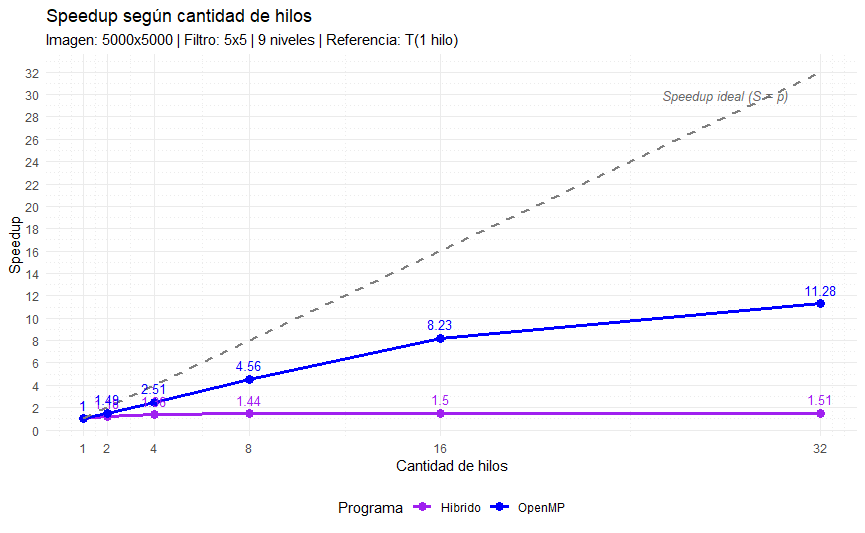
\includegraphics[width=0.9\textwidth]{../resources/Speedup_threads.png}
    \caption{Speedup en función de la cantidad de hilos para OpenMP e Híbrido. La línea punteada representa el speedup ideal ($S = p$). Configuración: imagen $5000 \times 5000$, filtro $5 \times 5$, 9~niveles.}
    \label{fig:speedup_threads}
\end{figure}

La curva de OpenMP (línea azul) exhibe un crecimiento sostenido y consistente a lo largo de todo el rango evaluado. Con 2~hilos se obtiene un speedup de $1{.}49$, lo que indica que prácticamente la totalidad del trabajo se distribuye efectivamente entre ambos hilos, con una pérdida mínima por overhead de creación del equipo de hilos. Al pasar a 4~hilos el speedup asciende a $2{.}51$, manteniendo una progresión cercana a la linealidad. El salto más significativo se produce al escalar a 8~hilos ($S = 4{.}56$), punto en el cual la curva comienza a separarse visiblemente de la línea de speedup ideal ($S = p$). La brecha entre la curva real y el speedup ideal demuestra el impacto de la fracción secuencial del algoritmo, acceso simultáneo a memoria, y el overhead propio de sincronización OpenMP.

La versión Híbrida (línea púrpura) presenta un comportamiento radicalmente distinto. Si bien con 2~hilos por nodo logra un speedup de $1{.}18$ respecto de su propia ejecución con 1~hilo, la curva se aplana casi por completo a partir de 4~hilos, estabilizándose en un rango estrecho entre $1{.}44$ y $1{.}51$ para todas las configuraciones de 4 a 32~hilos. Este estancamiento se explica por la latencia de la comunicación entre los 4~nodos MPI.


\subsection{Eficiencia según cantidad de hilos}

\begin{figure}[H]
    \centering
    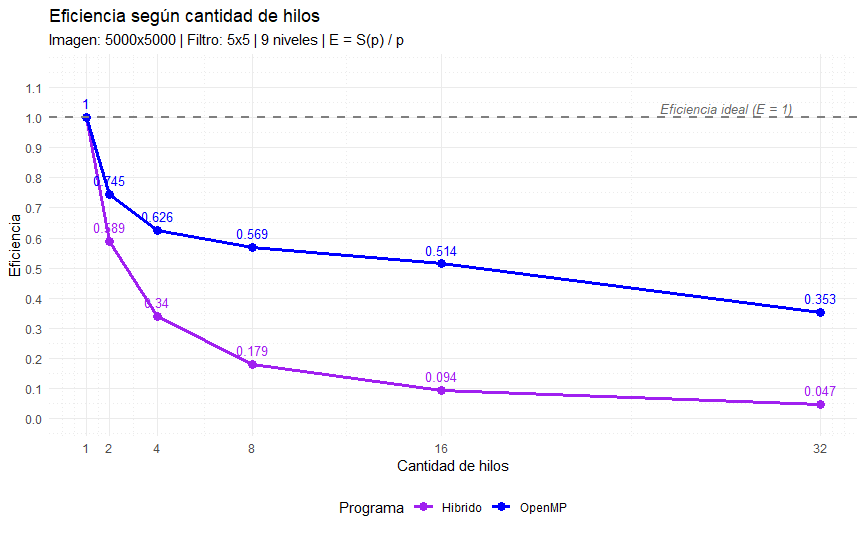
\includegraphics[width=0.9\textwidth]{../resources/Eficiencia_threads.png}
    \caption{Eficiencia en función de la cantidad de hilos para OpenMP e Híbrido. La línea punteada representa la eficiencia ideal ($E = 1$). Configuración: imagen $5000 \times 5000$, filtro $5 \times 5$, 9~niveles.}
    \label{fig:eficiencia_threads}
\end{figure}

OpenMP exhibe una degradación monótona pero controlada a medida que se incrementa la cantidad de hilos. Con 2~hilos la eficiencia se mantiene en $0{.}745$ (el $74{.}5\%$ del recurso agregado se aprovecha), desciende a $0{.}626$ con 4~hilos, y continúa cayendo de manera gradual hasta estabilizarse en $0{.}353$ con 32~hilos. El hecho de que con 32~hilos aún se conserve un $35{.}3\%$ de eficiencia confirma que el pipeline de procesamiento de imágenes posee una fracción paralela dominante, y que las decisiones de diseño adoptadas fueron efectivas.

En contraste, la versión Híbrida muestra una caída de eficiencia considerablemente más pronunciada. Desde un valor inicial de $0{.}589$ con 2~hilos, la eficiencia se desploma a $0{.}34$ con 4~hilos y continúa descendiendo hasta alcanzar apenas $0{.}047$ con 32~hilos por nodo (aprovechamiento del $4{.}7\%$). Esta degradación acelerada se explica por la asimetría inherente al modelo híbrido. A medida que el cómputo local se vuelve más rápido (aumento de hilos OpenMP), la fracción del tiempo total que se fue por la comunicación en red crece, haciendo que cada thread adicional aporte una mejora cada vez menor.
    \chapter{Conclusiones}

El desarrollo de este proyecto integrador nos permitió contrastar de forma empírica cuatro paradigmas de programación paralela aplicados a un problema real de procesamiento de imágenes, revelando tanto las fortalezas como las limitaciones inherentes a cada modelo, y al enfrentarse a diferentes escalas de cómputo. Los principales aprendizajes se sintetizan a continuación.

\begin{itemize}
    \item \textbf{OpenMP demostró ser la arquitectura más eficiente}, debido a la ausencia total de latencia de comunicación en red, y aprovechando al máximo los 32~núcleos disponibles dentro de un único nodo. Nuestra elección de planificación estática, combinada con la política de \textit{first-touch} para la asignación de memoria en arquitecturas NUMA, permitió maximizar la localidad caché y eliminar prácticamente todo el \textit{overhead} de sincronización entre threads.
    \item \textbf{MPI puro sufrió una penalización altísima por su inherente comunicación}. Con 128~núcleos intercambiando mensajes de forma simultánea, la comunicación entre procesos generado por las operaciones de \texttt{MPI\_Scatterv}, \texttt{MPI\_Gatherv} y el intercambio de halos inhibió el beneficio de la paralelización en la mitad de las configuraciones evaluadas. La alta variabilidad observada en los tiempos de ejecución entre iteraciones (con picos que casi duplicaban el tiempo secuencial) constituyen un factor imposible de predecir y controlar en entornos distribuidos.
    \item \textbf{El modelo Híbrido se posicionó como la solución más equilibrada}, combinando poca comunicación entre procesos (4~procesos MPI) con un máximo aprovechamiento de recursos (32~hilos OpenMP por nodo). Si bien sus valores absolutos fueron modestos comparados con OpenMP, la versión Híbrida superó consistentemente tanto al modelo secuencial como a MPI puro en todas las configuraciones, siendo la alternativa más escalable cuando el problema excede la capacidad de un solo nodo.
    \item Al variar gradualmente la cantidad de hilos de 1 a 32 sobre la configuración más exigente ($5000 \times 5000$, filtro de $5 \times 5$, 9~niveles), \textbf{OpenMP confirmó su dominio como paradigma paralelo}. La versión Híbrida, en cambio, demostró que la comunicación de red entre los 4~nodos MPI es un bottleneck.
    \item Del análisis de eficiencia se obtiene que aumentar la cantidad de núcleos solo se traduce en mejora computacional cuando la fracción paralela del algoritmo domina sobre la fracción de comunicación y sincronización.
\end{itemize}



    % -------------------------------------------------------------------
    % Bibliography/References  -  Harvard Style was used in this report
    % -------------------------------------------------------------------
    % \bibliography{references}  %  Patashnik, O. (1988), BibTEXing. Documentation for general BibTEX users.

    
\end{document}